\chapter{Complex Analysis}
\label{chap:complex-analysis}

Complex Analysis is the branch of math that deals with calculus for complex functions. It is a very intuitive field, sharing many similarities with real analysis (calculus for real functions) and with vector calculus. It's techniques, particularly the Residue theorem, are very important in QFT, so we provide a summary of them.

We restrict ourselves to a subclass of complex functions called \emphi{analytical} or sometimes \emphi{holomorphic} functions. These functions are continuous and infinitely differentiable functions of a single complex variable $z$. Examples of \textit{non}-analytical functions are 
$$z^*z,\qquad |z|,\qquad \mathrm{piecewise\ functions}.$$
We can express this requirement of analyticity in another way: if we write a complex number $z=a+bi$ as a vector $\bm z = (a, -b)^T$, then a function $f(z)$ being holomorphic is equivalent to the function $\bm f(\bm z)$ being curl-free and divergence-free in the vector calculus sense:
\begin{e}
  \nabla \cdot \bm f = 0\qquad \nabla \times \bm f = 0.
\end{e}

Despite this restriction, many functions are analytical and obey several very useful theorems concerning power series (section \ref{sec:ca-series}) and integration (section \ref{sec:ca-residue}).

\section{Series, Poles, and Branch Cuts}
\label{sec:ca-series}

It is a fact that all analytical functions can be written as a Taylor series which converges in some disk of radius $R$ centered on $z_0$:
\begin{e}
  f(z) = \sum_{n=0}^\infty \frac{(z-z_0)^n}{n!}\eval{\frac{d^n f}{d z^n}}_{z=z_0} \mathrm{\ converges\ for\ all\ }|z-z_0| < R.
\end{e}
In some functions (called \emphi{entire} functions), that disk is the entire complex plane, but for most functions the disk can only grow so large before the series diverges. The maximum radius of the disk, called the \emphi{radius of convergence} $R$, is always the distance to the nearest singularity of the function.

A \emphi{singularity} is a location where the function is undefined. The most common singularity is a \emphi{pole}, where $f$ blows up due to dividing by a small number. For example, the function $f(z)=1/z$ has a pole at $z=0$. $1/z^2$ also has a pole at zero, but we would call this a pole of multiplicity two due to the square in the denominator.

The relationship between series and poles is very useful, and sheds light on why some Taylor series of real functions diverge. For example, the function
\begin{e}
  f(x) = \frac{1}{x^2+1}
\end{e}
is defined for all real $x$, but its Taylor series centered on $x_0=0$ diverges at $x=\pm 1$. That is, it has a radius of convergence 1. We can see why by promoting $x$ to a complex variable $z$. Then $f(z)$ has poles at $z=\pm i$, since $1/(i^2+1)$ diverges. The distance between the center of the Taylor series ($0$) and the pole ($i$) is one, so $R=1$.

A series diverging is not always disastrous. Consider $f(z) = \ln{z}$, defined as the function such that $e^f(z) = z$. This function has a pole at $z=0$, since $e^{-\infty} = 0$. For this reason, the Taylor series around $z_0=1$ has a radius of convergence of $R=1$
\begin{e}
  \ln(1+z) = z-\frac{z^2}{2}+\frac{z^3}{3}-\frac{z^4}{4}+\dots - (-1)^n\frac{z^n}{n}.
  \label{eqn:log-expansion-0}
\end{e}
However, we can extend the domain of this function by evaluating the series at a new point, such as $z_1 = \ln ((1 + i)/\sqrt{2})$. Since $z_1$ is well within the radius of convergence of \ref{eqn:log-expansion-0}, we can also find all the derivatives of $\ln(z_1)$ and write out the Taylor series:
\begin{e}
  \ln(z) = \sum_{n=0}^\infty a_n (z-z_1)^n
\end{e}
where $a_n$ are new complex constants. Since the only pole of the logarithm is at $z=0$, this function has a radius of convergence of 1, and we can repeat the same trick for a new point, such as $z_2 = i$. With this technique, $\ln z$ can be defined with a Taylor series at every point in the complex plane (except $z=0$), despite the pole!\footnote{Note that we do not have a single Taylor series which works for every point; you must chose the right Taylor series which is centered on a nearby point.} This technique is called \emphi{analytic continuation}, and can be performed on any analytical function. A diagram is given in Figure \ref{fig:ln-analytic-continuation}.

\begin{figure}
  \centering
  \begin{tikzpicture}[scale=1.3]
    \draw (0,-3) -- (0,3);
    \draw (-3,0) -- (3,0);
    \draw [thick] (1,0) circle (1);
    \draw [thick] (0.707,0.707) circle (1);
    \draw [thick] (0,1) circle (1);
    \filldraw [black] (1,0) circle (2pt) node[anchor=south]{$z_0$};
    \filldraw [black] (0.707,0.707) circle (2pt) node[anchor=north east]{$z_1$};
    \filldraw [black] (0,1) circle (2pt) node[anchor=west]{$z_2$};
    \filldraw [black] (0,0) circle (2pt);
    \path [draw=black,snake it](-3,0) -- (0,0);
  \end{tikzpicture}
  \caption{Analytic continuation of $\ln z$ via Taylor series centered on $z_0$, $z_1$, and $z_2$. The dot in the center is the pole and the wavy line to the left is the branch cut.}
  \label{fig:ln-analytic-continuation}
\end{figure}

Qualitatively speaking, we've shown that the divergence of (\ref{eqn:log-expansion-0}) was a red herring except at $z=0$. The function was perfectly well defined.

Or was it? There is still one property left to check; if we analytically continue in some path that starts at $z=1$, encircles the origin, and comes back to $z=1$, do we reproduce the same value of $\ln 1$? Perhaps surprisingly, the answer to this question is no; originally $\ln 1 = 0$ but the analytically continued version states $\ln 1 = 2\pi$.\footnote{In the case of the logarithm, it is simple to find the $2\pi$ offset which analytical continuation produces. It happens that $\ln(re^{i\theta})$, where $r$ and $\theta$ are real, is $\ln r + i\theta$. Check this by exponentiating $\ln r + i\theta$ and confirming it is equal to $re^{i\theta}$. Then defining $z_i$ along a circle of radius $r=1$ keeps increasing the imaginary component of $z_i$ as $\theta$ is increased until the circle is complete and the analytical continuation has accumulated a $2\pi i$ offset.} It cannot be that $\ln 1 = 0$ and $2\pi$ at the same time.

This problem illustrates the weakness of analytical continuation. It allows a smooth function to be defined anywhere except at a pole, but it may induce inconsistencies like constant offsets in the value of the function. We fix these by defining a ``branch cut,'' which is an arbitrary path that connects to the simple pole and extends to infinity at which we say $\ln z$ is undefined. That way, the circular path used above to create an inconsistency is interrupted by the branch cut and the argument can no longer be made. This branch cut is represented with a wavy line in Figure \ref{fig:ln-analytic-continuation} and chosen to lie along the negative real axis by convention. In general, any pole in a function generated by analytical continuation should have a branch cut attached to it.For example, $\sqrt{z}$ also has a branch cut, conventionally chosen to lie along the negative real axis as well.

Awareness of the poles and branch cuts in a complex function is a crucial trick when it comes to Taylor expanding or integrating a function. The connection between integration and poles is worked out in the next chapter.


\section{Residue Theorem}
\label{sec:ca-residue}
This section is on the integrals of complex functions such as $f(z)$. Like in vector calculus, when we integrate a function $\int_\gamma dz\, f(z)$ we must specify a curve $\gamma$ and we define the integral in the usual way using Riemann sums. The parametrization of the curve is unimportant, but the location of the curve in complex space is. In vector calculus a two-dimensional vector field $\bm f(\bm z)$ obeys Green's theorem for integration around a closed contour $\gamma$:
\begin{e}
  \oint_\gamma \bm d\ell \cdot \bm f(\bm z) = \int_D d^2 \bm z\, \nabla \times \bm f(\bm z)
\end{e}
where $D$ is the interior of $\gamma$. If $\nabla \times \bm f(\bm z)=0$ everywhere, then the line integral is zero. We would say that $\bm f(\bm z)$ is \emphi{conservative}.

Analytical functions are also conservative in that 
\begin{e}
  \oint_\gamma dz\, f(z) = 0
  \label{eqn:complex-conservative}
\end{e}
when the complex function is defined everywhere inside $\gamma$. An equivalent statement is that one can move $\gamma$ in the complex plane and not change the value of the integral, as long as $f$ is defined everywhere that $\gamma$ was moved through. Both these statements are due to the connection between analytical functions and curl-free vector fields mentioned at the beginning of this section. However, the function might not be defined at a few poles $z_j$ within $\gamma$, and at these points we cannot use Green's theorem. Let us focus on these poles specifically now.

Suppose we have a function $f(z)=z^{-n}$, with a pole of multiplicity $n$ at the origin. We can find the value of a closed integral around the origin by integrating in a nearly-closed contour in a circle around the pole and taking a limit as the ends approach each other. Note that the radius of this circle doesn't matter because if we shrink or expand the circle to another radius, we do not pass the curve through any poles, so that the value of the integral doesn't change.

Complex functions obey the fundamental theorem of calculus:
\begin{e}
  \int_a^b dz\, f(z) = F(b)-F(a)\qquad \mathrm{where}\qquad \frac{dF}{dz} = f(z).
\end{e}
A function $F(z)$ is generally called an \emphi{antiderivative} of $f$.
We changed notation here by not specifying $\gamma$ and instead only specifying its endpoints. This is allowed because, as we just learned, $\gamma$ may be moved through space where $f$ is defined so its exact path doesn't matter.

An antiderivative of $z^{-n}$ is $F(z)=z^{1-n}/(1-n)$, just like for real $z$, except when $n=1$ in which case the antiderivative is $F(z)=\ln z$. For $n>1$, $F(z)$ is continuous so that $F(b)-F(a)\rightarrow 0$ as $b\rightarrow a$. It follows that the closed integral around $z^{-n}$ is zero for $n>1$. However, for $n=1$ we have to deal with the branch cut in the logarithm, over which $F(z)$ is \textit{dis}continuous. We've already mentioned that $F(z)$ increases by $2\pi i$ when moving counterclockwise over the branch cut, so that the value of $\int_a^b dz\, z^{-1}$ must likewise be $2\pi i$. To summarize,
\begin{e}
  \oint_a^b dz\, z^{-n} = \begin{cases}0 & n \neq 1 \\ 2\pi i & n = 1\end{cases}.
\end{e}

Returning to integrating an arbitrary function $f(z)$ with poles at $z_j$, by definition $f(z)$ can be expanded around a pole as follows:
\begin{e}
  f(z) = \frac{a_{-m}}{(z-z_j)^m} + \frac{a_{1-m}}{(z-z_j)^{m-1}} + \dots = \sum_{n=-m}^\infty a_n (z-z_j)^n.
\end{e}
The integral of this function is then zero for each term except $n=-1$, where it is $2\pi i a_{-1}$. We generally write the coefficient $a_{-1}$  of this Taylor series centered at $z_j$ as $a_{-1} = \Res f(z_j)$. Thus
\begin{e}
  \oint_\gamma dz f(z) = 2\pi i \sum_{z_j} \Res f(z_j)
  \label{eqn:residue-theorem}
\end{e}
where $z_j$ are the poles inside $\gamma$.

(\ref{eqn:residue-theorem}) is an incredibly powerful theorem. It can be used to integrate even very complicated functions over closed contours. It can even be used to perform integrals over non-closed contours, by extending the contour through some region of space where we know $f(z)$ is small until the contour becomes closed. For example, we can easily find that 
\begin{e}
  \int_{-\infty}^\infty \frac{dx}{1+x^2} = \pi
\end{e}
via the Residue theorem. First we split the integrand into partial fractions to find the residue:
\begin{e}
  \frac{1}{2}\int_{-\infty}^\infty dx \parens{\frac{i}{x+i} - \frac{i}{x-i}}.
\end{e}
The function has poles at $z=\pm i$, with $\Res f(i) = -i$ and $\Res f(-i)=i$. To make a closed curve, we can close the contour in an enormous loop with very large $|z|$ from the $+\infty$ of the real axis to the $-\infty$ side. This can be done over the real line, in which case the curve will run counterclockwise and enclose the $+i$ pole, or it can be done under the real axis in which case it will run clockwise and enclose the $-i$ pole. Both these answers should be consistent, and they are. The two poles have opposite residues, but integrating over a clockwise curve flips the sign of the integral so that the result for both is
\begin{e}
  \int_{-\infty}^\infty \frac{dx}{1+x^2} = 2\pi i \parens{\frac{1}{2}(-i)} = \pi.
\end{e}

\section{The Gamma Function}
\label{sec:ca-gamma}

We conclude our function on special analysis with the Gamma function, $\Gamma(z)$. $\Gamma(z)$ is one of many special functions, much like the Riemann zeta function $\zeta(z)$, which are discussed in conjunction with complex analysis because their properties are so much easier to understand in the context of complex variables. Nevertheless, when $\Gamma(z)$ appears in physics, a real argument is usually used.

The Gamma function is a crucial function that appears in QFT due to its relation to the surface area of a sphere, discussed in the next chapter. It is also relevant to statistics and can be helpful in computing miscellaneous integrals as well. It is a generalization of the factorial:
\begin{e}
  \Gamma(n+1) = n!
\end{e}
for integer $n$. A consistent definition that works for all $\Re z > 0$ is 
\begin{e}
  \Gamma(z) = \int_0^\infty dt\, t^{1-z} e^{-t}.
  \label{eqn:gamma}
\end{e}
One can check that this definition is consistent with the factorial by showing that 
\begin{e}
  \Gamma(x+1)=x\Gamma(x)
  \label{eqn:gamma-recursion}
\end{e}
and $\Gamma(0)$, which are also properties of factorials. The proof of this fact and other properties of the Gamma function are left to other books.

(\ref{eqn:gamma}) defines a Gamma function is analytic and smoothly connects all the values of the factorial on the positive real axis. Using analytical continuation, we can extend the function to the negative real axis, where it has poles at every negative integer and at zero (Figure \ref{fig:gamma}). At the zero pole, $\Gamma(z)$ has a convenient expansion:
\begin{e}
  \Gamma(\epsilon) = \frac{1}{\epsilon} - \gamma_E + \mathcal{O}(\epsilon)
\end{e}
which generalizes to 
\begin{e}
  \Gamma(-n + \epsilon) = \frac{(-1)^n}{n!}\parens{\frac{1}{\epsilon} - \gamma_E + \sum_{j=1}^n\frac{1}{j}} + \mathcal{O}(\epsilon)
\end{e}
where $\gamma_E \approx 0.57721$ is the Euler-Mascheroni constant.

\begin{figure}
  \centering
  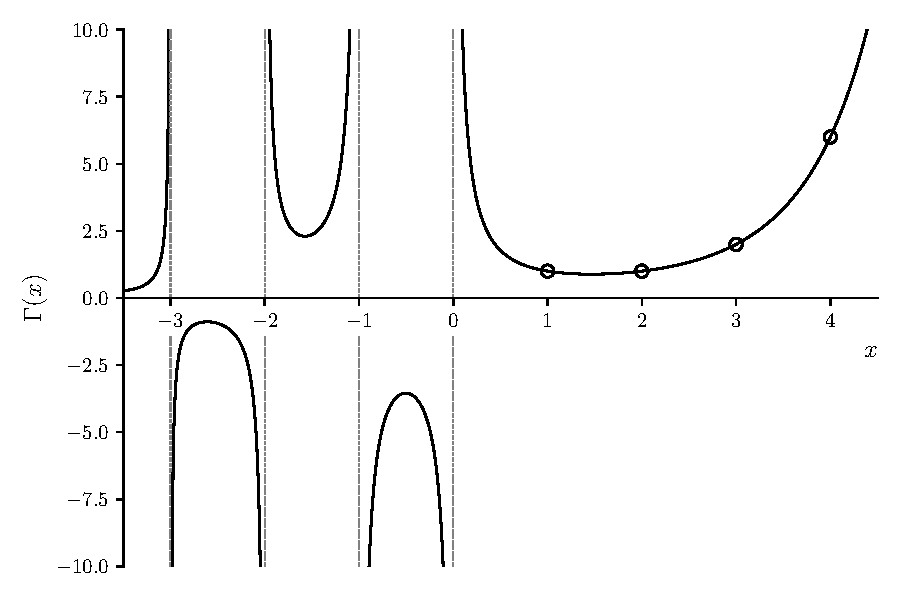
\includegraphics[width=\linewidth]{figs/gamma.pdf}
  \caption{The Gamma function, $\Gamma(x)$ on the real line. Open circles represent the value of $(x+1)!$, and dotted vertical lines are the poles at every non-positive integer.}
  \label{fig:gamma}
\end{figure}

Another useful formula is the values of the Gamma function at half-integers:
\begin{e}
  \Gamma\parens{z+\frac{1}{2}} = \frac{\sqrt{\pi}}{4^{z-\frac{1}{2}}}\frac{\Gamma(2z)}{\Gamma(z)}
\end{e}
which reduces to the special case of $\Gamma(\frac{1}{2}) = \sqrt{\pi}$. The Gamma function can also be used to aid in evaluating the following integral 
\begin{e}
  B(a,b) = \int_0^1 dt\, t^{a-1} (1-t)^{b-1}
  \label{eqn:beta-function}
\end{e}
which is called the \emphi{Beta function}. It appears in QFT as well as in probability and various trigonometric functions. It is related to the Gamma function via
\begin{e}
  B(a,b) = \frac{\Gamma(a)\Gamma(b)}{\Gamma(a+b)}.
  \label{eqn:beta-to-gamma}
\end{e}
Below, we use the Beta and Gamma functions to compute the surface area of a $d$-dimensional sphere.

\subsection{Surface Area of Spheres}
In physics, integrals over quantities which are rotationally symmetrical are very common. Such integrals can be separated into a radial part and an angular part, even in an arbitrary $d$-dimensional space, by integrating over $d$-dimensional spheres like so
\begin{e}
  \int d^d x\, f(|x|) = \parens{\int dr\, r^{d-1} f(r)}A_d
  \label{eqn:radial-integral}
\end{e}
where $A_d$ is the surface area of the $d$-dimensional unit sphere. For example, for $d=3$, we have $A_d = 4\pi$ and in $d=2$ we have $A_d=2\pi$.

The task of this section is to find the surface area of this $d$-dimensional sphere as a function of $d$, which we will do via recursion. Suppose we know the area $A_{d-1}$. This knowledge allows us to ignore all the $d-1$ axes of this sphere and project them down into a single axis $\hat x$, with the $d$th axis $\hat y$ being perpendicular to $\hat x$. Now we can think two-dimensionally.

\begin{figure}
  \centering
  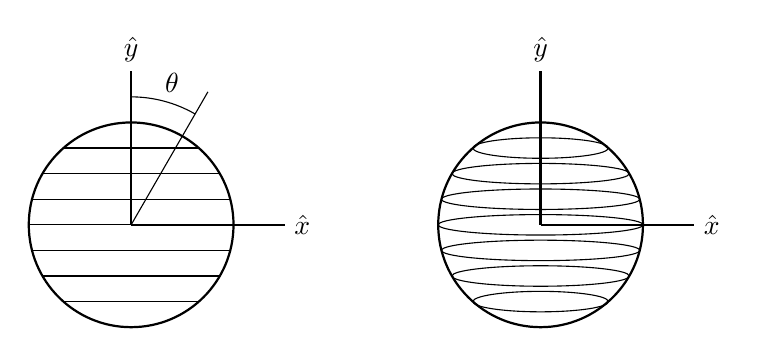
\begin{tikzpicture}[scale=1.3]
    \draw [thick] (-2,0) circle (1);
    \draw [thick] (-2,0) -- (-2,1.5);
    \draw [thick] (-2,0) -- (-0.5,0);
    \draw (-2,0) -- (-1.25,1.29903810567665);
    \draw (-2,1.25) arc (90:60:1.25);
    \draw (-1.6,1.2) node[anchor=south] {$\theta$};
    \draw (-2,1.5) node[anchor=south] {$\hat y$};
    \draw (-0.5,0) node[anchor=west] {$\hat x$};
    \draw (-3,0) -- (-1,0);
    \draw (-2.968245836551854,0.25) -- (-1.0317541634481457,0.25);
    \draw (-2.8660254037844384,0.5) -- (-1.1339745962155614,0.5);
    \draw (-2.6614378277661475,0.75) -- (-1.3385621722338523,0.75);
    \draw (-2.968245836551854,-0.25) -- (-1.0317541634481457,-0.25);
    \draw (-2.8660254037844384,-0.5) -- (-1.1339745962155614,-0.5);
    \draw (-2.6614378277661475,-0.75) -- (-1.3385621722338523,-0.75);


    \draw [thick] (2,0) circle (1);
    \draw [thick] (2,0) -- (2,1.5);
    \draw [thick] (2,0) -- (3.5,0);
    \draw (2,1.5) node[anchor=south] {$\hat y$};
    \draw (3.5,0) node[anchor=west] {$\hat x$};
    \draw (2, 0) ellipse (1 and 0.1);
    \draw (2, 0.25) ellipse (0.9682458365518543 and 0.1);
    \draw (2, 0.5) ellipse (0.8660254037844384 and 0.1);
    \draw (2, 0.75) ellipse (0.6614378277661475 and 0.1);
    \draw (2, -0.25) ellipse (0.9682458365518543 and 0.1);
    \draw (2, -0.5) ellipse (0.8660254037844384 and 0.1);
    \draw (2, -0.75) ellipse (0.6614378277661475 and 0.1);
  \end{tikzpicture}
  \caption{Stacking $d-1$-dimensional spheres to form a $d$-dimensional sphere for $d=2$ (\textit{left}) and $d=3$ (\textit{right}).}
  \label{fig:sphere-surface-area}
\end{figure}

The $d$-dimensional unit sphere corresponds to a unit circle on the $\hat x$ and $\hat y$ axes, which we parameterize by the angle $\theta$ between some point on the circle and the positive $\hat y$ axis. The $d$-dimensional unit sphere is created by stacking many $d-1$-dimensional spheres horizontally on top of each other like vertical lines inside the circle, meaning that the radius of one of these $d-1$-spheres is $r=\sin\theta$. It contributes an area of $dA = A_{d-1}\sin^{d-2}\theta d\theta$ to the total area. The $\sin^{d-2}\theta$ is present because surface area of the $d-1$ dimensional non-unit sphere is $A_{d-1}$ (the unit sphere area) times the radius to the $d-2$th power. This integration scheme is shown in Figure \ref{fig:sphere-surface-area}. Thus, the $d$-sphere surface area is 
\begin{es}
  A_d &= A_{d-1}\int_0^\pi d\theta\,\sin^{d-2}\theta \\
  &= -A_{d-1}\int_0^\pi d(\cos\theta)\,\sin^{d-3}\theta\\
  &= A_{d-1}\int_{-1}^1 dx\,\parens{1-x^2}^{\frac{d-3}{2}}\\
  &= A_{d-1}\int_0^1 dt\,t^{-\frac{1}{2}}\parens{1-t}^{\frac{d-3}{2}}
\end{es}
where in the second line we substituted variables from $\theta \rightarrow \cos\theta$, in the third line we expressed $\sin\theta = \sqrt{1-\cos^2\theta}$, and in the last line we substituted variables $x^2 \rightarrow t$. The reader may recognize the last integral as a Beta function $B(\frac{1}{2}, \frac{d-1}{2})$, so we may immediately write it in terms of $\Gamma$ functions:
\begin{e}
  A_d = A_{d-1} \frac{\Gamma\parens{\frac{1}{2}}\Gamma\parens{\frac{d-1}{2}}}{\Gamma\parens{\frac{d}{2}}} = A_{d-1} \sqrt{\pi}\frac{\Gamma\parens{\frac{d-1}{2}}}{\Gamma\parens{\frac{d}{2}}}.
\end{e}
Now we must turn the above recursive equation into a formula for $A_d$, but fortunately this is not difficult due to the $\Gamma$ function's own recursion relation (\ref{eqn:gamma-recursion}). The following formula checks out:
\begin{e}
  A_d = \frac{2\pi^{d/2}}{\Gamma\parens{\frac{d}{2}}}.
  \label{eqn:surface-area-sphere}
\end{e}

(\ref{eqn:surface-area-sphere}) draws a fascinating and unexpected connection between the Gamma function, which descended from factorials, and spheres. Without extending the factorials to the half-integers via the Gamma function, we could not have written (\ref{eqn:surface-area-sphere}) down.